\chapter{Static Linear Model}\label{c:linear}

One very common model for the static response of a system is the familiar equation of a line
\begin{equation}\label{e:line}
y = m*x+b
\end{equation}
where $x$ is the input, $y$ is the output, $m$ is the slope and $b$ is the y-intercept.  To put this in context of the dynamic linear models (e.g., first and second order) this model is referred to as a zero-order differential equation
\begin{equation}\label{e:zero}
y(t) = m*x(t)+b.
\end{equation}

One example of a physical system that can be approximated using this type of model is a mass-spring-damper idealization as shown in Figure~\ref{f:msd}.  We can consider either the dynamic response (which we'll model later as a second-order model) or the static response.  The static response ($x(t)$) to an input force ($F(t)$ of such a system can be approximated by Hooke's law
\begin{equation}\label{e:hooke}
x(t) = 1/K*F(t)
\end{equation}
where $K$ is the spring constant for the spring, $x(t)$ is the static displacement and $F(t)$ is the constant applied force.  Keep in mind that this is only reasonable for the \emph{static} scenario; if $F(t)$ is not constant this will be a very poor model to predict the response $x(t)$.

\begin{figure}[htb!]
\centerline{
{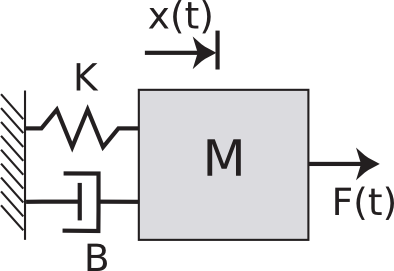
\includegraphics[width=0.4\textwidth]{msd_icon.png}}}
\caption{Sketch of a mass-spring-damper system.}
\label{f:msd}
\end{figure}


\section{Static Calibration}
In order to use a model such as (\ref{e:hooke}) we need to know the unknown parameters in the model, for example the spring constant $K$.  Static calibration is the process of experimentally determining this value.  If we know that the system is perfectly linear (which systems never are) and that our measurements are perfect (which they never are) this process is very simple.  All we have to do is...
\begin{itemize}
\item Apply a known static load $F$
\item Measure the resulting static displacement $x$
\item Substitute these values into (\ref{e:hooke}) and solve for $K$
\end{itemize}
This works surprisingly well if we are confident of our model (linearity) and our measurements.  However, to be a little more cautious we might want to repeat this process a few times at various known static loads and then combine all that data to determine a best-fit value for $K$ based on more than one measurement.  This process is known as \emph{fitting a model to the data}.

\section{Least-Squares Regression}
Regression analysis can be used to \emph{fit} model to experimental data.  For regression analysis the static model is a polynomial of order $m$ such as
\begin{equation}\label{e:rmodel}
\hat{y} = a_0+a_1*x+a_2*x^2+\ldots+a_m*x^m
\end{equation}
where $\hat{y}$ is the response predicted by the model.  Consider the linear case ($m=1$) illustrated in Figure~\ref{f:linear} where the model takes the form
\begin{equation}
\hat{x} = a_0 + 1/K*F
\end{equation}
and the experimental measurements are $x_i$ for each input $F_i$.  

\begin{figure}[hb!]
\centerline{
{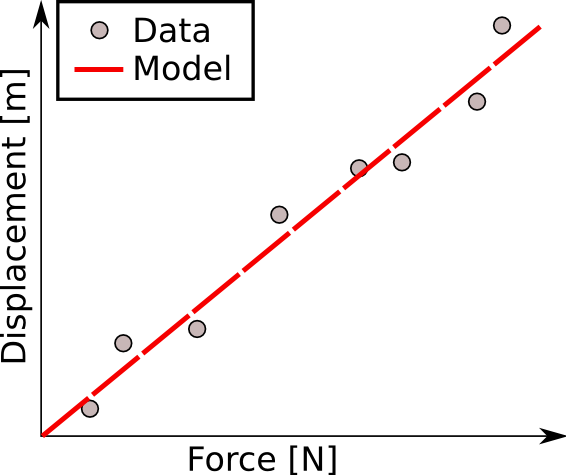
\includegraphics[width=0.4\textwidth]{linear_model_fit.png}}}
\caption{Illustration of a set of experimental measurements (data) and the best-fit linear model.}
\label{f:linear}
\end{figure}


In this case there are eight data points so $i=1,2,\ldots,8$.  The most common method to determine a the parameters of the model that best-fit the data is to minimize square-error between the prediction and the measurement at each test input.  In other words, the \emph{method of least-squares} finds values for $a_0$ and $K$ to minimize the quantity
\begin{equation}
L = \sum_{i=1}^N \left(x_i - \hat{x}_i \right)^2.
\end{equation}


Exactly how to accomplish this is beyond the scope of this book, but there are many tools (MATLAB, MS-Excel, etc.) that will solve this problem and provide you with a quantification of the \emph{goodness-of-fit}.  The first of these parameters is the \emph{coefficient of determination}, $R^2$, which defines, ``how much of the variance in the data is described by the linear fit''.  The $R^2$ parameter is between 0--1, with values greater than 0.9 indicated a good degree of fit (or agreement) between the data and the model.  Another way to quantify the comparison between the model and the data is to compute the \emph{standard error of the fit} as
\begin{equation}\label{e:standerror}
s = \sqrt{\frac{\sum_{i=1}^N \left(x_i - \hat{x}_i \right)^2}{\nu}}
\end{equation}
where $\nu$ is the degrees of freedom of the fit and $\nu=N-(m+1)$.  For our linear example ($m=1$) with eight data points ($N=8$), $\nu=8-(2)=6$. 
